\documentclass{standalone}
    \usepackage{tikz}
    \usepackage{pgfplots}
    \usetikzlibrary{calc}
    \usetikzlibrary{patterns}
    \usetikzlibrary{arrows}
\mathversion{bold}
\begin{document}
\huge
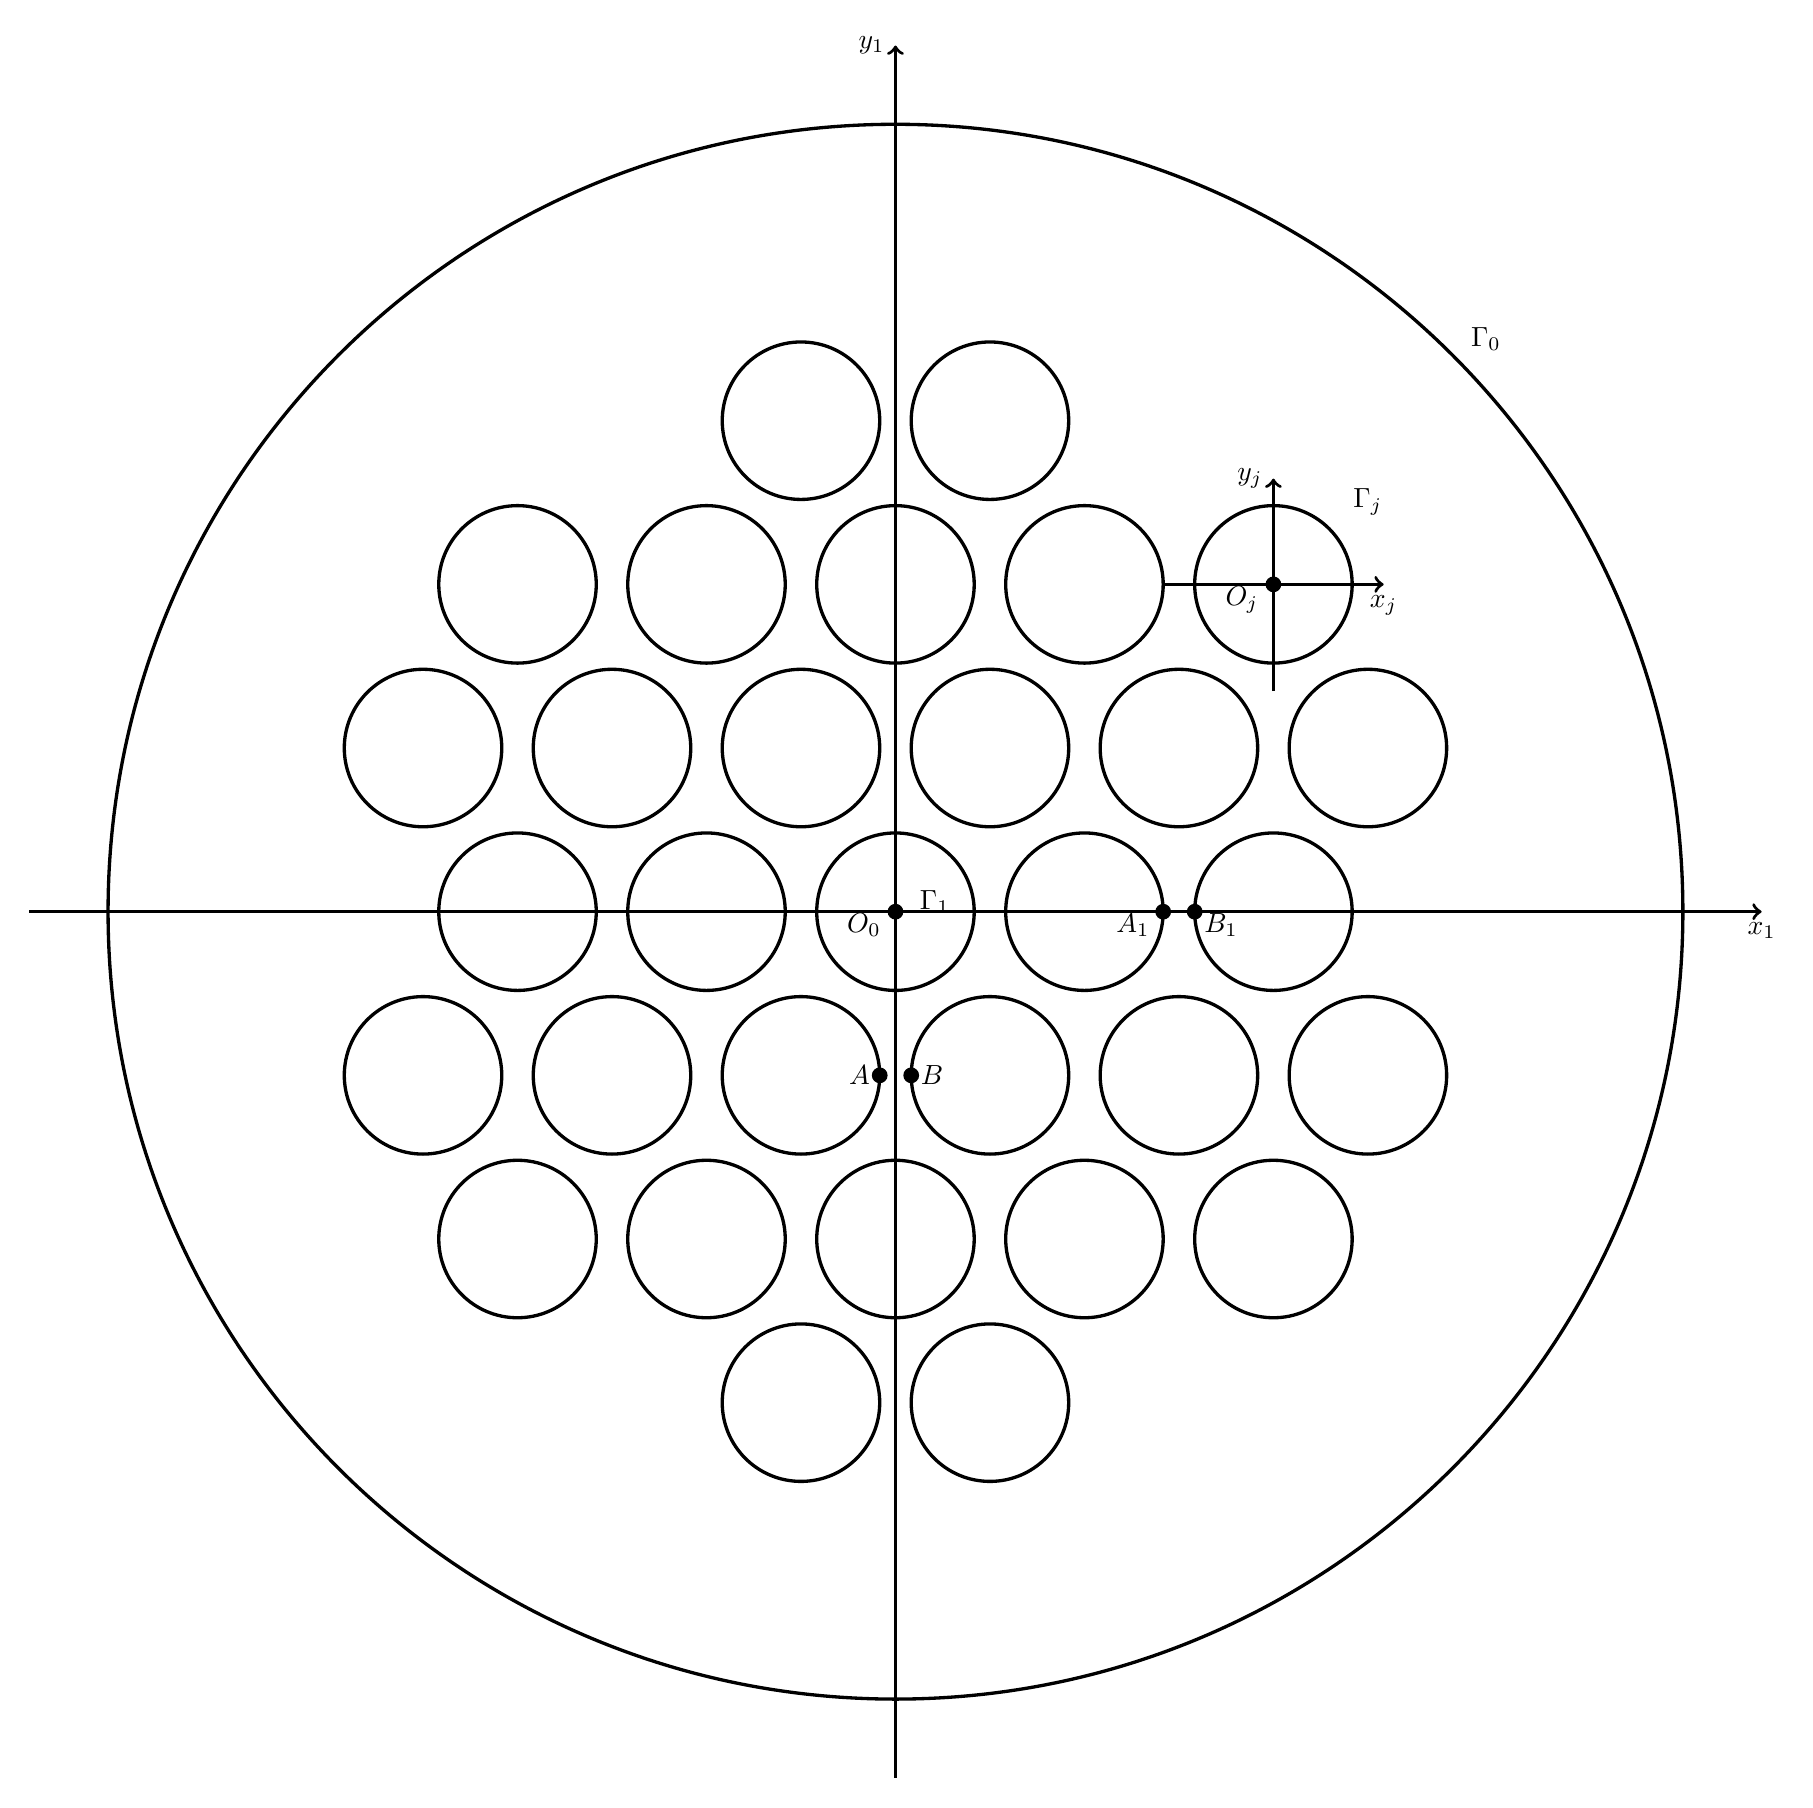
\begin{tikzpicture}
\coordinate (O) at (0,0);
\coordinate (O1) at (2.4, 0);
\coordinate (O2) at (1.2, 2.07846);
\coordinate (O3) at (-1.2, 2.07846);
\coordinate (O4) at (-2.4, 0);
\coordinate (O5) at (-1.2, -2.07846);
\coordinate (O6) at (1.2, -2.07846);
\coordinate (O7) at (6., 2.07846);
\coordinate (O8) at (4.8, 4.15692);
\coordinate (O9) at (2.4, 4.15692);
\coordinate (O10) at (4.8, 0.);
\coordinate (O11) at (1.2, 6.23538);
\coordinate (O12) at (-1.2, 6.23538);
\coordinate (O13) at (-2.4, 4.15692);
\coordinate (O14) at (-4.8, 4.15692);
\coordinate (O15) at (-6., 2.07846);
\coordinate (O16) at (-4.8, 0.);
\coordinate (O17) at (-6., -2.07846);
\coordinate (O18) at (-4.8, -4.15692);
\coordinate (O19) at (-2.4, -4.15692);
\coordinate (O20) at (2.4, -4.15692);
\coordinate (O21) at (-1.2, -6.23538);
\coordinate (O22) at (1.2, -6.23538);
\coordinate (O23) at (6., -2.07846);
\coordinate (O24) at (4.8, -4.15692);
\coordinate (O25) at (0, 0);
\coordinate (O26) at (3.6, 2.07846);
\coordinate (O27) at (0, 4.15692);
\coordinate (O28) at (-3.6, 2.07846);
\coordinate (O29) at (-3.6, -2.07846);
\coordinate (O30) at (0, -4.15692);
\coordinate (O31) at (3.6, -2.07846);


\coordinate (A) at (-0.2, -2.07846);
\coordinate (B) at (0.2, -2.07846);
\coordinate (C) at  (-1.4, 0);
\coordinate (D) at (1.4, 0);
\coordinate (A1) at (3.4, 0);
\coordinate (B1) at (3.8, 0);
\coordinate (C1) at (2.2, 2.07846);
\coordinate (D1) at (5.0, 2.07846);

\draw[very thick] (O) circle (10.0);
\draw[->,very thick] (-11,0) -- (11,0) node[below] {$x_1$};
\draw[->,very thick] (0,-11) -- (0,11) node[left] {$y_1$};

\draw[->,very thick] (3.4,4.15692) -- (6.2,4.15692) node[below] {$x_j$};
\draw[->,very thick] (4.8,2.8) -- (4.8,5.5) node[left] {$y_j$};

\draw[very thick] (O1) circle (1.0);
\draw[very thick] (O2) circle (1.0);
\draw[very thick] (O3) circle (1.0);
\draw[very thick] (O4) circle (1.0);
\draw[very thick] (O5) circle (1.0);
\draw[very thick] (O6) circle (1.0);
\draw[very thick] (O7) circle (1.0);
\draw[very thick] (O8) circle (1.0);
\draw[very thick] (O9) circle (1.0);
\draw[very thick] (O10) circle (1.0);
\draw[very thick] (O11) circle (1.0);
\draw[very thick] (O12) circle (1.0);
\draw[very thick] (O13) circle (1.0);
\draw[very thick] (O14) circle (1.0);
\draw[very thick] (O15) circle (1.0);
\draw[very thick] (O16) circle (1.0);
\draw[very thick] (O17) circle (1.0);
\draw[very thick] (O18) circle (1.0);
\draw[very thick] (O19) circle (1.0);
\draw[very thick] (O20) circle (1.0);
\draw[very thick] (O21) circle (1.0);
\draw[very thick] (O22) circle (1.0);
\draw[very thick] (O23) circle (1.0);
\draw[very thick] (O24) circle (1.0);
\draw[very thick] (O25) circle (1.0);
\draw[very thick] (O26) circle (1.0);
\draw[very thick] (O27) circle (1.0);
\draw[very thick] (O28) circle (1.0);
\draw[very thick] (O29) circle (1.0);
\draw[very thick] (O30) circle (1.0);
\draw[very thick] (O31) circle (1.0);

\fill (A) circle (0.1);
\fill (B) circle (0.1);
\fill (O8) circle (0.1);
\fill (O25) circle (0.1);
%\fill (D) circle (0.1);
\fill (A1) circle (0.1);
\fill (B1) circle (0.1);
%\fill (C1) circle (0.1);
%\fill (D1) circle (0.1);
\node[left] at (A) {$A$};
\node[right] at (B) {$B$};
%\node[above right] at (C) {$C$};
%\node[above left] at (D) {$D$};
\node[below left] at (3.35,0.1) {$A_1$};
\node[below right] at (3.8,0.1) {$B_1$};
\node[below] at (4.4,4.25) {$O_j$};
\node[below] at (6,5.5) {$\Gamma_j$};
\node[below] at (-0.4,0.1) {$O_0$};
\node[above] at (0.5,-0.15) {$\Gamma_1$};
\node[above] at (7.5,7) {$\Gamma_0$};

\end{tikzpicture}
\end{document}

%%% Local Variables: 
%%% mode: latex
%%% TeX-master: t
%%% End: 
